\subsubsection{Configurazione scrittura del ricalcolo della rete}
\begin{figure} [H]
	\centering
	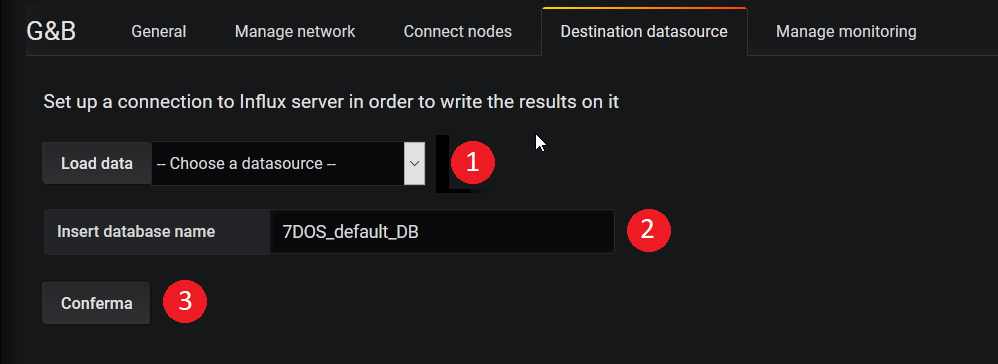
\includegraphics[scale=0.55]{Img/setds} 
	\caption{Tab di configurazione scrittura del ricalcolo della rete} \label{} 
\end{figure} 
La configurazione dei parametri di scrittura avviene tramite i seguenti step:
\begin{enumerate}
	\item Scelta della datasource;
	\item Indicazione del database di scrittura;
	\item Conferma dei parametri.
\end{enumerate}

N.B. In caso di mancata selezione di una datasource o di un database, verranno selezionati i parametri di default (cioè il datasource di default indicato all'interno di Grafana e il database "7DOS\_defaultDB").